\begin{table}[htbp]\centering\small
\caption{Accuracy and hit diagnostics for explicitly named reports. Panel A reports paired working-reference tests; Panel B uses the fixed nonoverlap grid for hit tests. A better average score does not imply fewer breaches.}\label{sup:old-diagnostics}
\begin{tabular}{>{\raggedright\arraybackslash}p{4.3cm}>{\raggedright\arraybackslash}p{2.1cm}>{\raggedright\arraybackslash}p{2.1cm}>{\raggedright\arraybackslash}p{5.7cm}}\toprule
Panel A: paired contrast & DM p & HLN p & Named adjustment / p\\\midrule
FX original main comparison & 2.20e-07 & 2.31e-07 & Two-main comparison Bonferroni: 4.39e-07\\
FX matched history & 4.47e-09 & 4.83e-09 & Original matched Holm family: 2.86e-07\\
Treasury original main comparison & 0.00761 & 0.00939 & Original matched Holm family: 0.320\\
\bottomrule\end{tabular}
\par\smallskip\begin{minipage}{.98\linewidth}\footnotesize Original matched Holm uses 72 contrasts. The later regrouped matched family is separate; earlier-period writing-stage HAC comparisons have neither a new HLN field nor a new family adjustment.\end{minipage}

\par\medskip\begin{center}\small
\begin{tabular}{p{4.0cm}rrrr}\toprule
Panel B: report & Grid hits & Grid issues & Kupiec p & Christoffersen CC p\\\midrule
FX regression & 50 & 947 & 0.695 & 0.636\\
FX original rolling reference & 49 & 947 & 0.807 & 0.905\\
FX matched fixed reference & 49 & 947 & 0.807 & 0.646\\
Treasury regression & 7 & 40 & 0.00413 & 0.0136\\
Treasury historical reference & 4 & 40 & 0.199 & 0.262\\
\bottomrule\end{tabular}\end{center}
{\footnotesize Hit tests use the full fixed nonoverlap grid; the conditional-coverage likelihood conditions on its initial hit. Equality to the nominal tail rate is the stated diagnostic null, distinct from the population upper-quantile inequality. The grid does not create independence.}
\end{table}

\begin{figure}[htbp]\centering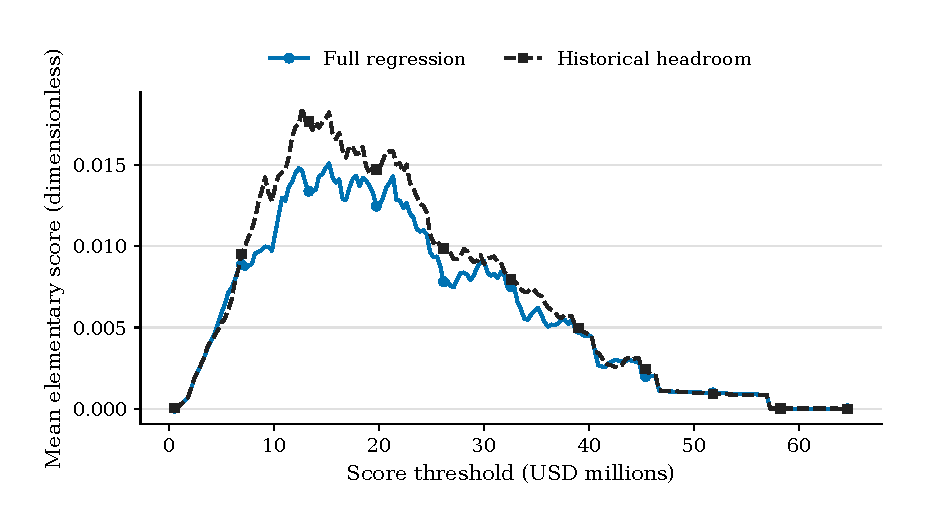
\includegraphics[width=.94\linewidth]{figures/v7-murphy-fx_hourly.pdf}
\caption{Murphy diagram for the main short-horizon FX comparison. The full-breakpoint calculation finds crossings; the graph is a display of saved scores. Average pinball superiority does not imply dominance across elementary scores.}\label{fig:murphyfx}
\end{figure}

\begin{figure}[htbp]\centering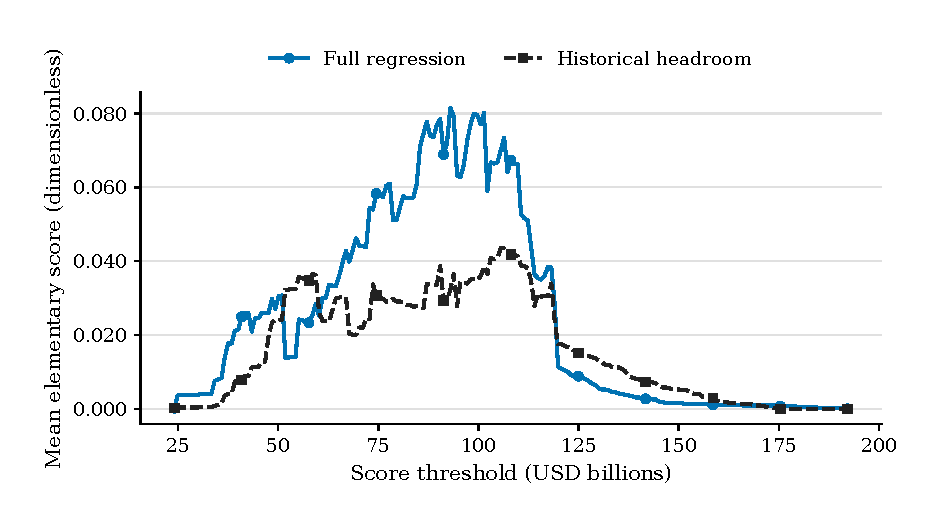
\includegraphics[width=.94\linewidth]{figures/v7-murphy-nyfed_weekly.pdf}
\caption{Murphy diagram for the main Treasury-bill comparison. The saved full-breakpoint comparison also crosses. A single average-score ordering leaves other consistent-score preferences unresolved.}\label{fig:murphybill}
\end{figure}
